\chapter{The Forensic Dashboard}
\label{ch:dashboard}

The benchmark scheduler (Chapter~\ref{ch:scheduler}) and metrics pipeline
(Chapter~\ref{ch:metrics}) produce hundreds of JSON files---one per suite,
per run, per role.  To make this data \emph{useful}, researchers need a
visual tool that loads, cross-references, and charts the results.  This
chapter describes the \textbf{Forensic Dashboard}: a web application that
turns raw benchmark data into interactive charts, tables, heatmaps, and
anomaly reports.

\begin{keyinsight}
The dashboard is a \emph{forensic} tool, not a real-time monitor.  It loads
pre-recorded benchmark runs, not live data.  Its motto (displayed in the UI)
captures this philosophy: ``No smoothing.  No causal inference.  Raw
observational forensic data.''
\end{keyinsight}

% ============================================================
\section{Technology Stack}
\label{sec:dash-stack}

\begin{table}[htbp]
\centering
\caption{Dashboard technology stack}
\label{tab:dash-stack}
\begin{tabular}{@{}l l p{6cm}@{}}
\toprule
\textbf{Layer} & \textbf{Technology} & \textbf{Purpose} \\
\midrule
Backend   & Python / FastAPI    & REST API, data loading, anomaly detection \\
Models    & Pydantic v2         & Typed request/response schemas \\
Frontend  & React 18 + TypeScript & Interactive UI components \\
State     & Zustand             & Lightweight global state management \\
Charts    & Recharts            & Bar, scatter, pie, and line charts \\
Styling   & Tailwind CSS        & Utility-first CSS framework \\
Build     & Vite                & Fast development server and bundler \\
\bottomrule
\end{tabular}
\end{table}

\begin{analogy}
If the benchmark scheduler is the robot lab technician that runs experiments,
the dashboard is the research notebook where you spread out the results,
highlight anomalies, and compare measurements side by side.
\end{analogy}

% ============================================================
\section{Backend Architecture}
\label{sec:dash-backend}

The backend is a FastAPI application (version~3.0) with CORS support for local
development.  It serves data through a RESTful API consumed by the React
frontend.

\subsection{Data Loading: The MetricsStore}

The \texttt{MetricsStore} class (in \texttt{dashboard/backend/ingest.py})
loads benchmark data from exactly three scenario folders:

\begin{table}[htbp]
\centering
\caption{Scenario folder mapping}
\label{tab:dash-scenarios}
\begin{tabular}{@{}l l p{5.5cm}@{}}
\toprule
\textbf{Folder} & \textbf{Run Type} & \textbf{Description} \\
\midrule
\texttt{runs/no-ddos/}        & \texttt{no\_ddos}       & Baseline: clean network \\
\texttt{runs/ddos-xgboost/}   & \texttt{ddos\_xgboost}  & DDoS with XGBoost detection \\
\texttt{runs/ddos-txt/}       & \texttt{ddos\_txt}      & DDoS with text-based rules \\
\bottomrule
\end{tabular}
\end{table}

Each folder contains per-suite JSON files (the output of the
\texttt{MetricsAggregator}).  The store:

\begin{enumerate}
  \item Scans each scenario folder for \texttt{*.json} files.
  \item Parses filenames to extract suite ID, run ID, and role
        (drone or GCS).
  \item Loads each file into a \texttt{ComprehensiveSuiteMetrics} Pydantic
        model (v2, mirroring the 18-category schema).
  \item Merges time-adjacent drone and GCS records into a single consolidated
        suite entry.
  \item Indexes entries by composite key \texttt{\{run\_id\}:\{suite\_id\}}.
  \item Builds per-run summaries (\texttt{RunSummary}) with suite counts,
        timestamps, and hostnames.
\end{enumerate}

\begin{designdecision}
Only these three scenario folders feed the dashboard.  Old runs, broken logs,
and intermediate files are ignored.  This strict scoping prevents stale or
malformed data from polluting the analysis.
\end{designdecision}

\subsection{Pydantic Models}

The file \texttt{dashboard/backend/models.py} defines Pydantic v2 models that
mirror the 18-category schema:

\begin{itemize}
  \item 18 nested model classes (one per category A--R), each with typed
        \texttt{Optional} fields matching the dataclass schema.
  \item \texttt{ComprehensiveSuiteMetrics}: the top-level model containing
        all 18 categories plus an \texttt{ingest\_status} field for
        provenance tracking.
  \item \texttt{SuiteSummary}: a lightweight projection with key fields
        (suite ID, KEM, SIG, AEAD, handshake duration, power, pass/fail).
  \item \texttt{RunSummary}: per-run metadata (ID, start time, suite count,
        hostnames).
\end{itemize}

\subsection{API Endpoints}

Table~\ref{tab:dash-api} lists the principal API endpoints.

\begin{table}[htbp]
\centering
\caption{Dashboard API endpoints}
\label{tab:dash-api}
\begin{tabular}{@{}l l p{5cm}@{}}
\toprule
\textbf{Endpoint} & \textbf{Method} & \textbf{Purpose} \\
\midrule
\texttt{/api/suites}          & GET  & List suites with optional filters \\
\texttt{/api/suite/\{key\}}   & GET  & Full metrics for one suite \\
\texttt{/api/runs}            & GET  & List all benchmark runs \\
\texttt{/api/filters}         & GET  & Available filter values (KEM, SIG, AEAD, level) \\
\texttt{/api/anomalies}       & GET  & Anomaly detection results \\
\texttt{/api/settings}        & GET  & Dashboard settings (labels, active runs, thresholds) \\
\texttt{/api/settings/\ldots} & POST & Update labels, active runs, or thresholds \\
\texttt{/api/multi-run/compare}   & GET & Cross-run comparison for one suite \\
\texttt{/api/multi-run/overview}  & GET & Aggregated KPIs per active run \\
\texttt{/api/metric-semantics}    & GET & Per-field provenance and type info \\
\bottomrule
\end{tabular}
\end{table}

\subsection{Settings Store}

Dashboard settings (run labels, active run selection, anomaly thresholds) are
persisted in a local JSON file.  The \texttt{SettingsStore} class provides
atomic read/write with defaults.  Settings include:

\begin{itemize}
  \item \textbf{Run labels}: Human-readable names and scenario types for
        each run ID.
  \item \textbf{Active runs}: Up to~3 runs selected for multi-run comparison.
  \item \textbf{Anomaly thresholds}: Warning/critical thresholds for
        handshake duration (ms), packet loss ratio, power deviation (\%),
        and energy deviation (\%).
\end{itemize}

% ============================================================
\section{Frontend Architecture}
\label{sec:dash-frontend}

The frontend is a single-page React application built with Vite and TypeScript.

\subsection{Application Layout}

The \texttt{App.tsx} component defines a fixed left sidebar (navigation) and a
scrollable main content area.  The sidebar groups 12 routes into four
categories:

\begin{table}[htbp]
\centering
\caption{Dashboard navigation structure}
\label{tab:dash-nav}
\begin{tabular}{@{}l l l@{}}
\toprule
\textbf{Group} & \textbf{Page} & \textbf{Route} \\
\midrule
Overview  & Dashboard        & \texttt{/} \\
\addlinespace
Analysis  & Suite Explorer   & \texttt{/suites} \\
          & Bucket Comparison & \texttt{/bucket} \\
          & Suite Comparison & \texttt{/compare} \\
          & Multi-Run Compare & \texttt{/multi-run} \\
\addlinespace
Metrics   & Power \& Energy  & \texttt{/power} \\
          & Latency \& Transport & \texttt{/latency} \\
          & Security Impact  & \texttt{/security} \\
          & Integrity Monitor & \texttt{/integrity} \\
\addlinespace
Config    & Metric Semantics & \texttt{/semantics} \\
          & Settings         & \texttt{/settings} \\
\bottomrule
\end{tabular}
\end{table}

\subsection{State Management: Zustand Store}

All application state lives in a single Zustand store (\texttt{store.ts}).
Key state slices include:

\begin{description}
  \item[Data] Suites list, runs list, selected suite(s), comparison data.
  \item[Settings] Dashboard configuration, active runs, anomaly thresholds.
  \item[Anomalies] Detected anomalies scoped to the latest run.
  \item[Filters] KEM family, SIG family, AEAD algorithm, NIST level, run ID.
  \item[UI] Loading indicator, error messages.
\end{description}

The store exposes 18~actions that fetch data from the backend API, update
local state, and push settings changes back to the server.

\subsection{TypeScript Type System}

The file \texttt{types.ts} mirrors the backend's 18-category schema as
TypeScript interfaces.  Each Pydantic model maps to a corresponding interface
(e.g.\ \texttt{RunContextMetrics}, \texttt{CryptoPrimitiveBreakdown},
\texttt{PowerEnergyMetrics}), ensuring type safety from the API boundary
all the way to the chart components.

Additional utility types include \texttt{AnomalyItem}, \texttt{SuiteFlag},
\texttt{DashboardSettings}, and a \texttt{RunType} enum with three values
(\texttt{no\_ddos}, \texttt{ddos\_xgboost}, \texttt{ddos\_txt}).

% ============================================================
\section{Dashboard Pages}
\label{sec:dash-pages}

\subsection{Overview (Dashboard)}

The landing page provides an executive summary:

\begin{itemize}
  \item \textbf{9~KPI cards}: Total suites, pass rate, average handshake
        (with P95 and $\sigma$), average power, anomaly count, fastest/slowest
        suite, average goodput, total energy.
  \item \textbf{3~pie charts}: Distribution of suites by NIST level, KEM
        family, and SIG family.
  \item \textbf{Scatter chart}: Handshake duration vs.\ energy, colour-coded
        by NIST level---revealing the cost/security trade-off at a glance.
  \item \textbf{Bar charts}: Average handshake, power, goodput, and packet
        loss grouped by KEM family.
  \item \textbf{Scenario status banner}: Shows which of the three scenario
        folders are present, with run and suite counts.
  \item \textbf{Multi-run comparison cards}: Per-run KPIs for side-by-side
        comparison across scenarios.
  \item \textbf{Benchmark runs table}: All runs with metadata (ID, scenario,
        start time, hosts, git commit).
\end{itemize}

\subsection{Suite Explorer}

A filterable, heatmap-coloured table of all cipher suites:

\begin{itemize}
  \item Five dropdown filters (run, KEM, SIG, AEAD, NIST level).
  \item Each row shows suite ID, algorithms, handshake timing, power, energy,
        pass/fail status, and anomaly indicator.
  \item Numeric cells use a green-to-red gradient based on the value's
        position within the column's range.
  \item Clicking a suite navigates to the detail page.
\end{itemize}

\subsection{Suite Detail}

A comprehensive deep-dive into a single suite's full metric inventory:

\begin{itemize}
  \item Metric cards organised by schema section (A, B, D, G, H, K, N, O, P,
        F, R).
  \item Each value carries a \textbf{reliability badge}
        (\textsc{verified}, \textsc{conditional}, \textsc{deprecated},
        \textsc{missing}) and a \textbf{consistency classification}
        (\textsc{consistent}, \textsc{broken}, \textsc{misleading}).
  \item A full metric inventory table showing every key/value with status,
        source (drone/GCS), and origin function.
  \item Expandable raw JSON payloads for the drone record, GCS record, and
        GCS validation JSONL.
\end{itemize}

\subsection{Latency Analysis}

Deep dive into transport-layer timing:

\begin{itemize}
  \item 6~KPI cards: average RTT, jitter, one-way latency, handshake,
        goodput, packet loss (each with P95).
  \item Per-NIST-level KPI breakdown.
  \item Grouped bar charts (handshake + RTT + jitter by KEM family; by NIST
        level).
  \item Scatter chart: handshake vs.\ RTT with bubble size $\propto$ power.
  \item Top-20 suites table with 13 columns.
\end{itemize}

\subsection{Security Impact}

Anomaly detection dashboard:

\begin{itemize}
  \item 4~KPI cards: critical anomalies, warnings, clean suites, total suites.
  \item Horizontal bar chart: anomaly count by metric name.
  \item Stacked bar chart: critical vs.\ warning by KEM family.
  \item Flagged-suites table with severity badges and per-flag details.
\end{itemize}

The security impact page is designed to highlight which suites behave
anomalously under DDoS conditions compared to the baseline run.

\subsection{Power Analysis}

Power and energy visualisation:

\begin{itemize}
  \item 4~KPI cards: average power (W), total energy (J), suites with power
        data, sensor type.
  \item Bar chart: energy by KEM family.
  \item Scatter chart: power vs.\ handshake duration (bubble size $\propto$
        energy).
  \item Top-10 energy consumers table.
\end{itemize}

\subsection{Comparison View}

Side-by-side comparison of two selected suites:

\begin{itemize}
  \item Two dropdown selectors (Suite~A as baseline, Suite~B).
  \item Horizontal bar chart comparing 6~metrics (handshake, goodput, packet
        loss, power, energy, CPU).
  \item Detailed comparison table with 8~rows of key metrics.
\end{itemize}

This page answers questions like ``How does ML-KEM-512 with AES-GCM compare
to ML-KEM-1024 with ChaCha20 in handshake time and power?''

\subsection{Multi-Run Comparison}

Compares the \emph{same} suite across up to 3~benchmark runs (e.g.\ baseline
vs.\ DDoS scenarios):

\begin{itemize}
  \item Suite selector dropdown.
  \item Per-run metric cards showing the suite's performance under each
        scenario.
  \item Highlights differences caused by network conditions rather than
        cryptographic choice.
\end{itemize}

\subsection{Integrity Monitor}

Client-side data quality checks:

\begin{itemize}
  \item 4~KPI cards: clean suites, high/medium/low severity issues.
  \item Integrity checks:
    \begin{description}
      \item[High] Benchmark marked FAIL, handshake did not succeed.
      \item[Medium] Missing power data, handshake $> 10\,$seconds.
    \end{description}
  \item Issues table with severity badges and links to suite detail.
\end{itemize}

\subsection{Metric Semantics}

A reference page documenting every metric field in the schema:

\begin{itemize}
  \item Text filter by key name.
  \item Table with 8~columns: key, category, origin side (drone/GCS),
        authoritative side, nullable, zero-valid, legacy flag, observed types.
\end{itemize}

This page serves as the developer's dictionary for interpreting JSON fields.

\subsection{Settings}

Configuration interface:

\begin{itemize}
  \item Benchmark run checkboxes (activate up to 3 for multi-run comparison).
  \item Per-run label and type assignment.
  \item Scenario folder status display.
  \item Anomaly threshold editors (6~numeric inputs).
\end{itemize}

% ============================================================
\section{Data Flow: Backend to Frontend}
\label{sec:dash-flow}

\begin{figure}[htbp]
\centering
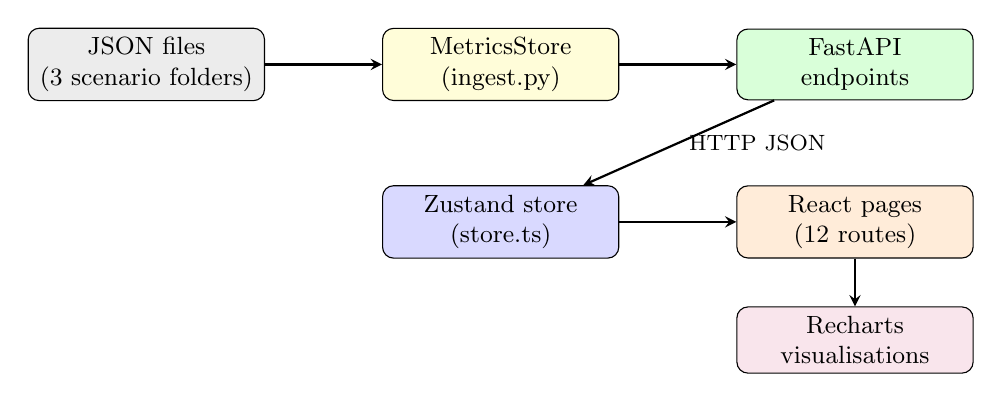
\begin{tikzpicture}[
    box/.style={draw, rounded corners, minimum width=3cm,
                minimum height=0.8cm, font=\small, align=center},
    arr/.style={->, >=stealth, thick}
  ]
  \node[box, fill=gray!15] (files) at (0,0) {JSON files\\(3 scenario folders)};
  \node[box, fill=yellow!15] (store) at (4.5,0) {MetricsStore\\(ingest.py)};
  \node[box, fill=green!15] (api) at (9,0) {FastAPI\\endpoints};
  \node[box, fill=blue!15] (zustand) at (4.5,-2) {Zustand store\\(store.ts)};
  \node[box, fill=orange!15] (pages) at (9,-2) {React pages\\(12 routes)};
  \node[box, fill=purple!10] (charts) at (9,-3.5) {Recharts\\visualisations};

  \draw[arr] (files) -- (store);
  \draw[arr] (store) -- (api);
  \draw[arr] (api) -- node[right, font=\footnotesize] {HTTP JSON} (zustand);
  \draw[arr] (zustand) -- (pages);
  \draw[arr] (pages) -- (charts);
\end{tikzpicture}
\caption{Data flow from benchmark output files through the backend API,
Zustand state management, React pages, and into Recharts visualisations.}
\label{fig:dash-flow}
\end{figure}

% ============================================================
\section{Anomaly Detection}
\label{sec:dash-anomaly}

The dashboard implements a threshold-based anomaly detection system.  For each
suite, it compares key metrics against configurable warning and critical
thresholds:

\begin{itemize}
  \item \textbf{Handshake duration}: Warning if $> T_w$ ms, critical if
        $> T_c$ ms (defaults: 5000\,ms / 30000\,ms).
  \item \textbf{Packet loss ratio}: Warning if $> L_w$, critical if $> L_c$
        (defaults: 0.01 / 0.05).
  \item \textbf{Power deviation}: Warning if the suite's power deviates from
        the population mean by more than $D_p$\,\%.
  \item \textbf{Energy deviation}: Warning if energy deviates by more than
        $D_e$\,\%.
\end{itemize}

Anomalies are computed server-side (scoped to the latest or selected run) and
returned as a list of \texttt{AnomalyItem} objects with severity, metric name,
observed value, threshold, and suite ID.  The Security Impact page visualises
these as bar charts and a flagged-suites table.

% ============================================================
\section{Chapter Summary}

\begin{itemize}
  \item The \textbf{Forensic Dashboard} is a FastAPI + React web application
        that visualises post-hoc benchmark data.
  \item The backend loads JSON files from 3~scenario folders (baseline,
        DDoS-XGBoost, DDoS-text), indexes them by run and suite, and serves
        them through a REST API.
  \item Pydantic v2 models mirror the 18-category metrics schema, ensuring
        type safety from disk to API.
  \item The React frontend uses Zustand for state, TypeScript for type safety,
        Recharts for visualisation, and Tailwind~CSS for styling.
  \item 12~pages cover the full analysis workflow: executive overview, suite
        exploration, latency deep-dive, power analysis, security anomalies,
        data integrity, cross-suite comparison, multi-run comparison, and
        metric reference documentation.
  \item Threshold-based \textbf{anomaly detection} flags suites with
        abnormal handshake times, packet loss, or power consumption.
\end{itemize}
